\documentclass[10pt,letterpaper]{article}
\usepackage[latin1]{inputenc}
\usepackage{amsmath}
\usepackage{amsfonts}
\usepackage{amssymb}
\usepackage{makeidx}
\usepackage{graphicx}
\usepackage{algorithm2e}
\usepackage[left=1.00in, right=1.00in, top=1.00in, bottom=1.00in]{geometry}
\author{Jay Ricco, David Van Chu}
\title{Introduction to Artificial Intelligence\\Project Update}
\date{Due: July 13, 2017}
\begin{document}
	\maketitle
	\section{Update}
		Binary Trees implementation is complete and David has began testing it with MNIST and CIFAR10 datasets.
		Jay ran into a setback with the Differentiable Boundary Trees portion of the project, and is currently implementing it using Torch rather than TensorFlow. If this is not completed by Tuesday, July 18th, we will pivot to focus on the existing Boundary Trees implementation. Meanwhile, David will continue testing the Boundary Trees:
		\begin{enumerate}
			\item Set a seed for random to make future results reproducable.
			\item Set the branching factor to different values.
			\item Calculate standard deviation along with averages.
			\item Find a way to visualize the datasets during training and testing.
		\end{enumerate}
		\subsection{DBT's Setback}
			Jay's issue was caused by the underlying computation architecture of TensorFlow. The compute graphs compiled by the library are static, while the algorithm requires dynamically building them. Implementation in PyTorch should be far easier and actually accurate. To date, the logical flow behind the implementation is as follows:\\
			\begin{algorithm}
				\SetAlgoLined
				$trainbatch$ = get\_mnist\_training\_batch(BATCH\_SIZE)\\
				$f_{\theta}$ = initialize\_feedforward\_compute\_graph()\\
				\For{$\left( tx, ty \right)$ $\in$ trainbatch}{Train Boundary Tree $\mathcal{T}$ using transform $f_{\theta}$}
				\For{$\left(tx, ty \right)$ $\in$ $\subset$ trainbatch}{Build Network Function $Net_{\theta}$ using 'Torchified' query function.\\
				Back-propagate error and update $\theta$ using $Net$} 
			\end{algorithm}
			
		\section{Backup Plan}
		If we decide to focus on the existing Boundary Trees implementation, we will test it with different distance functions to see how they perform on MNIST and CIFAR10. We will also create synthetic data sets to test speed as dataset size increases, without caring how accurate the boundary tree is.
	
	\section{Data Collected}
		So far, we have collected data using MNIST and CIFAR10 with (unintentionally) a branching factor set to infinity, essentially replicating k-nearest neighbors algorithm. Using all of the examples for each data set, the average accuracy for MNIST was 88.201\%, and for CIFAR10, 26.936\%. We expect that Differentiable Boundary Trees will be more accurate than Boundary Trees, especially with the CIFAR10 dataset. There may be other distance functions that improve the accuracy rate of CIFAR10 with regular Boundary Trees, and if we are not able to implement DBTs, then we will investigate other distance functions.
			\begin{figure}
			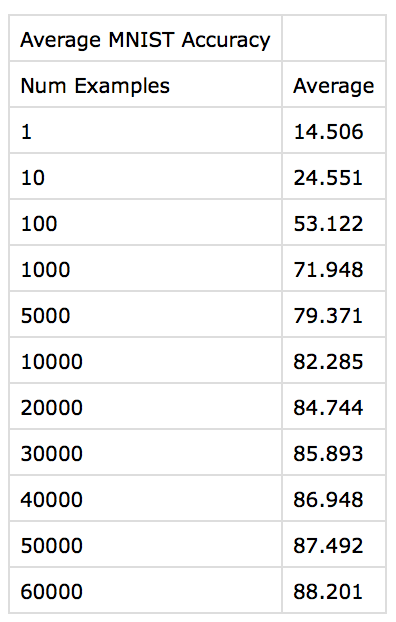
\includegraphics[width=150pt]{1.png}
			\caption{MNIST Averages.}
			\label{fig:1}
		\end{figure}
		\begin{figure}
			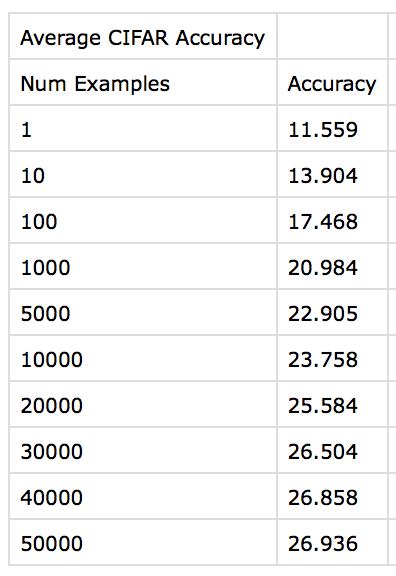
\includegraphics[width=150pt]{2.png}
			\caption{CIFAR Averages.}
			\label{fig:2}
		\end{figure}
\end{document}